\documentclass[12pt]{article}
\usepackage{geometry}
\geometry{
	left=20mm,
	top=20mm,
}
\usepackage[utf8]{inputenc}
\usepackage{array}
\newcolumntype{C}[1]{>{\centering\let\newline\\\arraybackslash\hspace{0pt}}m{#1}}
\usepackage[spanish]{babel}
 \usepackage{url}
\usepackage[spanish, fixlanguage]{babelbib}
\bibliographystyle{IEEEtran}
\usepackage{graphicx}
\graphicspath{ {./images/} }
\usepackage{amssymb}
\usepackage{amsmath}
\usepackage{subcaption}
\usepackage[linesnumbered]{algorithm2e}
\newcommand\mycommfont[1]{\footnotesize\ttfamily\textcolor{blue}{#1}}
\SetCommentSty{mycommfont}
\usepackage{tikz}
\usetikzlibrary{positioning, fit}
\usetikzlibrary{babel}
\usepackage{titlesec}
\titlespacing*{\section}
{0pt}{5.5ex plus 1ex minus .2ex}{.3ex plus .1ex}
\titlespacing*{\subsection}
{0pt}{5.5ex plus 1ex minus .2ex}{2.3ex plus .1ex}
\title{Tarea 6}

\author{
	Saul Ivan Rivas Vega \\
	\\
	Diseño y análisis de algoritmos\\
\\
	Equipo Completo:\\
		Yadira Fleitas Toranzo\\
		Diego de Jesús Isla Lopez\\
		Saul Ivan Rivas Vega\\
}

\date{\today}

\begin{document}
	\maketitle
	\pagebreak
	\section{}
	  \paragraph{} Sea $T$ un árbol binario con raíz y $S$ un conjunto con un número par de vértices de $T$. Diseña un algoritmo de tipo $divide-y-vencer\acute{a}s$ de tiempo $O(n)$ que empareje los nodos en $S$ de forma tal que en $T$ existan caminos disjuntos en aristas entre cada par.
	  \\ La figura siguiente muestra un ejemplo del problema en el $S$ tiene los seis vértices encerrados en círculos y los emparejamientos se denotan con tres tipos distintos de lineas punteadas.
	  \\
	  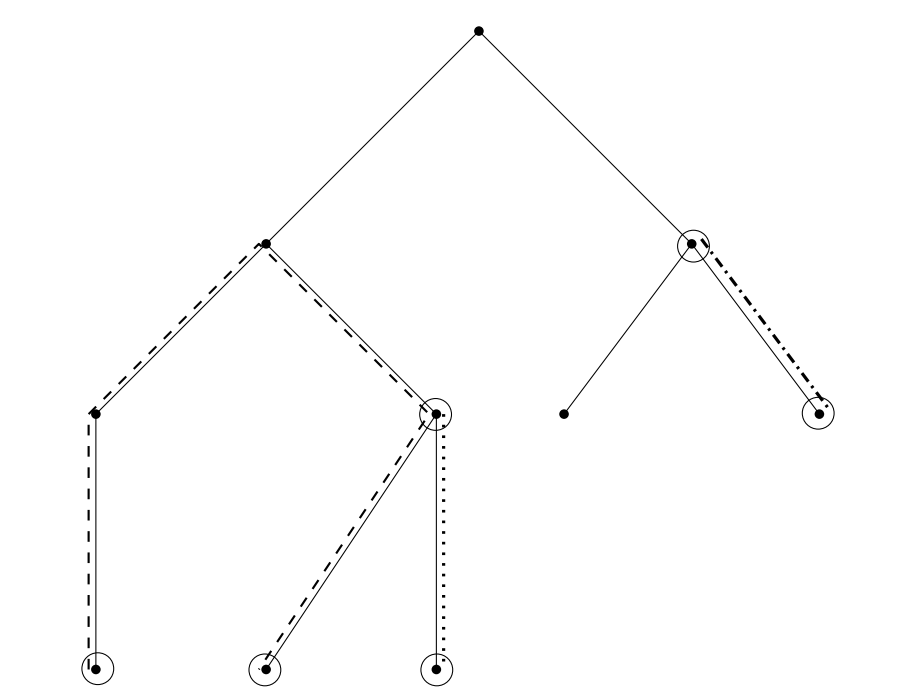
\includegraphics[width=\textwidth]{tree_1}
	  \pagebreak
\subsection{Algoritmo}
		\begin{algorithm}[H]\footnotesize
		\KwData{Árbol $T$, donde los nodos tienen adicionalmente un valor True o False si es que pertenecen al conjunto $S$.}
		\KwResult{Conjunto $R$ con las parejas.}
		\SetAlgoLined
		\tcc{Inicializar el conjunto $R$.}
		$R:=\{\}$\;
		\tcc{Llamar la función obtenerParejas' con la raíz del árbol y el conjunto respuesta.}
		obtenerParejas'(raíz, R)\;
		return $R$\;
		\caption{Algoritmo obtenerParejas.}
	\end{algorithm}
\begin{algorithm}[H]\footnotesize
	\KwData{Nodo $u$ y el conjunto actual de parejas $R$.}
	\KwResult{Un nodo que no fue emparejado en el subárbol de $u$, o un valor vacío si no existe dicho nodo.}
	\SetAlgoLined
	\tcc{Inicializar los valores de los nodos sin emparejar encontrados en el subárbol del hijo izquierdo y del hijo derecho, originalmente vacíos} 
	$nodo\_libre\_izq:=\emptyset$\;
	$nodo\_libre\_der:=\emptyset$\;
	\tcc{Realizamos llamadas recursivas en el subárbol del hijo izquierdo y derecho si es que existen} 
	\If{u tiene hijo izquierdo}{$nodo\_libre\_izq$:=obtenerParejas'(hijo izquierdo de $u$, $R$)}
	\If{u tiene hijo derecho}{$nodo\_libre\_der$:=obtenerParejas'(hijo derecho de $u$, $R$)}
	\tcc{Si no hay nodos por emparejar en los subárboles checamos si $u$ tiene que ser emparejado, si es el caso lo devolvemos como nodo por emparejar en su subárbol, en caso contrario devolvemos un valor vacío} 
	\If{$nodo\_libre\_izq$ y $nodo\_libre\_der$ son $\emptyset$}{
		\eIf{u esta en $S$}{
			return $u$\;
		}{return $\emptyset$\;}
	}
	\tcc{En este punto  hay al menos un nodo por emparejar en alguno de los subárboles izquierdo o derecho.} 
 	\tcc{Checamos si $u$ tiene que emparejarse.}
 	\If{u esta en $S$}{
	 	\tcc{Checamos si hubo un nodo libre en el subárbol izquierdo y si es el caso, emparejamos $u$ con ese nodo y devolvemos el valor de $nodo\_libre\_der$ que puede ser vacío o un nodo libre.}
		\eIf{$nodo\_libre\_izq$ no es igual a $\emptyset$}{
			agregamos la pareja $(u, nodo\_libre\_izq)$ a $R$\;
			return $nodo\_libre\_der$\;
		}{
		\tcc{En caso contrario, emparejamos $u$ con el nodo libre en el subárbol derecho y devolvemos un valor vacío.}
			agregamos la pareja $(u, nodo\_libre\_der)$ a $R$\;
			return $\emptyset$\;
		}
 	}
 \tcc{Checamos si existen ambos nodos de los subárboles para emparejarlos o en su defecto retornar el nodo que no este vacío.}
 	\If{no son vacíos $nodo\_libre\_izq$ y $nodo\_libre\_der$} {
 		agregamos la pareja $(nodo\_libre\_izq, nodo\_libre\_der)$ a $R$\;
 		return $\emptyset$
 	}
	return el nodo que no este vacío entre $nodo\_libre\_izq$ y $nodo\_libre\_der$\;
	\caption{Algoritmo obtenerParejas'.}
\end{algorithm}
\pagebreak
\subsection{Demostración complejidad $O(n)$}
El algoritmo 1 realmente no nos dice mucho, solo inicializa el conjunto respuesta y lo retorna al terminar $obtenerParejas'$ el cual es el segundo algoritmo. Por esta razón realizaremos el análisis en el segundo algoritmo.
Cuando el algoritmo es invocado en un nodo hoja, no se realizan mas llamadas recursivas.\\
Esto es, el algoritmo seguirá bajando en en árbol hasta llegar a una hoja, pues antes de realizar una llamada recursiva revisa si tiene un hijo izquierdo o derecho, como se observa en las líneas $3$ y $6$, como una hoja no tiene hijos pues se detendrá ahí.\\
\paragraph{Observación 1} El algoritmo es invocado en un nodo una única vez. Es decir, el algoritmo se llama sobre los hijos del nodo pero en ningún momento se realiza una llamada al padre o a un nodo que no este directamente conectado al nodo actual $u$. Así pues cuando el algoritmo pasa por el nodo $u$, no volveremos a procesar a $u$.\\
\paragraph{Observación 2} Las operaciones realizadas al ser invocado en una hoja, o al regresar de las llamadas recursivas, son de tiempo constante. Es decir que a partir de la línea $9$ hasta el final de las operaciones, solo se realizan comparaciones y asignaciones que podemos considerar de tiempo constante.   \\
Por la observación 1 podemos decir que como existen $n$ nodos, se realizarán $n$ veces las operaciones descritas en la Observación 2 y al ser de tiempo constante decimos que realizamos $n$ veces operaciones de tiempo constante. \\
Finalmente decimos que el algoritmo es de complejidad $O(n)$.
\subsection{Observación} Se pide solo el diseño del algoritmo con la complejidad $O(n)$ en el ejercicio pero se incluye una explicación de porque es correcto.
\paragraph{Correctitud.} 
El algoritmo termina pues por la Observación 1, no se realizarán mas llamadas recursivas al llegar a las hojas, y  en estas solo se toma en cuenta el if en la línea $9$ si es que devolvemos o no al nodo para emparejar. Siendo el número de llamadas $n$ y en cada llamada se realiza un número constante de operaciones.\\
\paragraph{Observación 3} En cada invocación se deja a lo más un nodo sin emparejar  en el subárbol con raíz $u$. Esto lo podemos demostrar por inducción.\\
\textbf{Invariante: } Se deja a lo más un nodo sin emparejar  en el subárbol con raíz $u$ al terminar una invocación.\\
\textbf{Caso base:} Se considera un subárbol de un solo nodo, es decir una hoja. En este caso se devuelve el valor del único nodo si es que tiene que ser emparejado. Se cumple la invariante pues solo podemos devolver el valor del nodo o un valor vacío.\\
\textbf{Hipótesis inductiva:} En cada invocación intermedia podemos emparejar los nodos libres que existan en el subárbol, de tal forma que dejemos a lo más uno libre.\\
Suponer verdadero hasta algún nodo intermedio en el árbol $T$.\\
Dicha invocación en el nodo $u$ tiene los siguientes casos:
\begin{enumerate}
	\item \textbf{u no tiene que emparejarse}
	\begin{enumerate}
		\item La invocación del hijo izquierdo si devolvió un valor no vacío y también la invocación en el hijo derecho. En este caso se emparejan dichos nodos y no quedan nodos libres.
		\item Alguna de las dos invocaciones en los hijos devolvió un valor no vacío y otro sí. En este caso queda libre el nodo que no fue vacío de las invocaciones.
		\item Ninguna de las dos invocaciones en los hijos devolvió un valor no vacío. En este caso no quedan nodos libres.
	\end{enumerate}
	\item \textbf{u si tiene que emparejarse}
	\begin{enumerate}
		\item La invocación del hijo izquierdo si devolvió un valor no vacío y también la invocación en el hijo derecho. En este caso se emparejan el nodo $u$ con el nodo libre de la invocación en el hijo izquierdo, dejando libre el nodo de la invocación en el hijo derecho.
		\item Alguna de las dos invocaciones en los hijos devolvió un valor no vacío y otro sí. En este caso se empareja la el nodo $u$ con el nodo libre de las invocaciones y no quedan nodos libres.
		\item Ninguna de las dos invocaciones en los hijos devolvió un valor no vacío. En este caso queda libre el nodo $u$.
	\end{enumerate}
\end{enumerate}
Finalmente como en ninguno de los casos se termina con dos o mas nodos libres podemos decir que en cada invocación se deja a lo más un nodo sin emparejar  en el subárbol con raíz $u$.
Probemos ahora que las parejas resultantes no comparten aristas en el camino que las conecta.\\
Por contradicción.\\
Entonces significa que hay por lo menos una arista por el cual pasan 2 caminos entre parejas. \\
Tomemos el subárbol $T_j$ el cuál tiene como raíz al nodo inferior en dicha arista. Tal como se muestra en la figura siguiente.\\
\begin{figure}[h]
\begin{center}
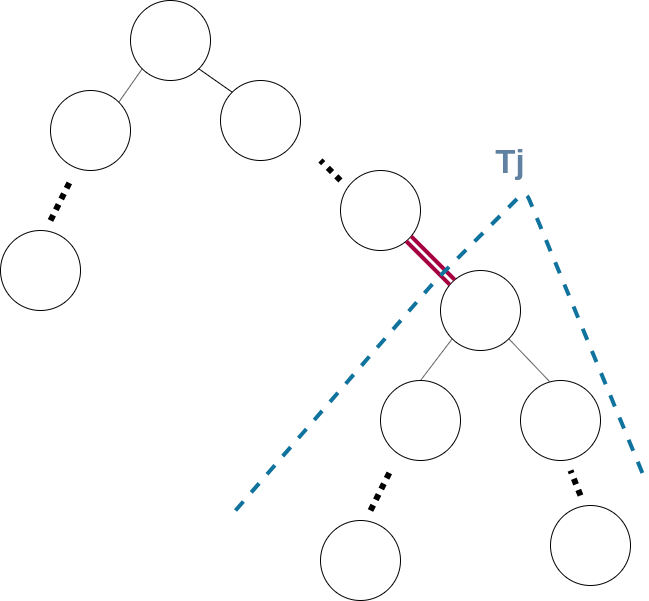
\includegraphics[scale=0.5]{ARBOL}
	\end{center}
\caption{Subárbol $T_j$ (línea punteada), arista con doble camino (en rojo).}
\end{figure}
\pagebreak
\paragraph{} En el subárbol $T_j$
\subsection{Calendarizar clases usando el mínimo número de salones de clases posibles.}
\begin{algorithm}[H]\small
	\KwData{Conjunto $C$ con clases, definidos por su tiempo de inicio y tiempo de termino.}
	\KwResult{Conjunto $P$ de conjuntos $T_{i}$ que contiene las clases para el salon $i$ donde $0<i \leq total\_de\_salones$.}
	\SetAlgoLined
	Insertar todos las clases $c \in C$ a una cola de prioridad $Q$ ordenando por c.tiempo\_inicio\;
	Inicializar una cola de prioridad adicional vacía $S$ para las clases por salón\;
	\tcc{La cola de priordad $S$ tendra parejas (clase, salon), ordenados por clase.tiempo\_termino.}
	\tcc{Inicializar el conjunto $P$ para la respuesta.}
	$P:=\{\}$\;
	\While{Q no este vacía}{
		Sacar la clase $c$ que este al frente de $Q$\;
    	\tcc{Inicializar el salon para la clase $c$.}
		salon\_clase\_c:=0\;
		\If{$S$ tiene elementos}{
			\tcc{No sacar el elemento al frente de $S$ solo obtener los valores.}
			(clase\_mas\_cercana, salon) := S.frente()\;
			\If{$c.tiempo\_inicio \geq clase\_mas\_cercana.tiempo\_termino$}{
				Sacar el elemento al frente de $S$\;
				salon\_clase\_c:=salon\;
			}
		}
	 \tcc{Si no se le asignó un salon entonces crear uno nuevo.}
		\If{salon\_clase\_c==0}{
    	   \tcc{Sera el número de salones actuales mas uno.}
			salon\_clase\_c:= S.tamano() + 1\;
		}
		\If{ no existe $P[salon\_clase\_c]$}{
			Inicializar $P[salon\_clase\_c]:=[]$\;
		}
		Insertar $c$ en $P[salon\_clase\_c]$\;
		Insertar $(c, salon\_clase\_c)$ en $S$\;
	}
	return $P$\;
	\caption{Algoritmo Calendarización de clases.}
\end{algorithm}
\paragraph{}
\pagebreak
\paragraph{Demostración complejidad $O(nlogn)$}
En una cola de prioridad las operaciones para insertar tiene complejidad $O(logn)$.\\
Al inicio se insertan los $n$ elementos en la cola de prioridad $Q$, realizando $n$ operaciones de inserción y como cada operación de inserción tiene complejidad $O(logn)$ tenemos que al terminar de insertarlos habremos realizado $nlogn$ operaciones.\\
En el ciclo $while$ realizaremos iteraciones mientras aún haya elementos en $Q$, y como en cada iteración sacamos al elemento $t$ que esta al frente. Es decir, el número de iteraciones es igual al número de elementos en $Q$. Al inicio insertamos a todos los trabajos en $Q$, siendo entonces $n$ iteraciones.\\
En cada iteración realizaremos las siguientes operaciones:\\
\begin{itemize}
	\item Sacar la clase $c$ al frente de $Q$, que es la operación de remover en una cola de prioridad, siendo de complejidad $O(logn)$.
	\item Sacar el elemento al frente de $S$, siendo $O(logn)$ en una cola de prioridad.
	\item Insertar $(c, salon\_clase\_c)$ en $S$, siendo $O(logn)$ en una cola de prioridad.
	\item Comparaciones y asignaciones que podemos considerar como de complejidad $O(1)$.
\end{itemize}
Como hacemos $n$ iteraciones entonces tenemos que el ciclo $while$ es de complejidad $O(nlogn)$. \\
Como tanto la parte inicial como el ciclo $while$ tienen la misma complejidad dominante, finalmente decimos que el algoritmo es de complejidad $O(nlogn)$.\\
\subsection{Calendarización para minimizar la latencia máxima.}
\begin{algorithm}[H]\small
	\KwData{Conjunto $T$ con trabajos, definidos por su tiempo requerido y su deadline.}
	\KwResult{Arreglo $S$ con los trabajos en el orden requerido para minimizar la latencia máxima.}
	\SetAlgoLined
	Insertar todos los trabajos $t \in T$ a una cola de prioridad $Q$ ordenando por t.deadline\;
	\tcc{Inicializar el conjunto $S$ para la respuesta.}
	$S:=\{\}$\;
	\While{Q no este vacía}{
		Sacar al trabajo $t$ que este al frente de $Q$\;
		insertar $t$ en $S$\;
	}
	return $S$\;
	\caption{Algoritmo minimizar la latencia máxima.}
\end{algorithm}

\paragraph{Demostración complejidad $O(nlogn)$}
En una cola de prioridad las operaciones para insertar tiene complejidad $O(logn)$.\\
Al inicio se insertan los $n$ elementos en la cola de prioridad $Q$, realizando $n$ operaciones de inserción y como cada operación de inserción tiene complejidad $O(logn)$ tenemos que al terminar de insertarlos habremos realizado $nlogn$ operaciones.\\
En el ciclo $while$ realizaremos iteraciones mientras aún haya elementos en $Q$, y como en cada iteración sacamos al elemento $t$ que esta al frente. Es decir, el número de iteraciones es igual al número de elementos en $Q$. Al inicio insertamos a todos los trabajos en $Q$, siendo entonces $n$ iteraciones.\\
En cada iteración además de remover un elemento de $Q$. Para la operación de remover a un elemento esta es de complejidad $O(logn)$ y como hacemos $n$ iteraciones entonces tenemos que el ciclo $while$ es de complejidad $O(nlogn)$. \\
Como tanto la parte inicial como el ciclo $while$ tienen la misma complejidad dominante, finalmente decimos que el algoritmo es de complejidad $O(nlogn)$.\\
\section{Ejercicio 2. Da un algoritmo de tipo $greedy$ para alguno de los siguientes problemas.}
Se escogió el problema:
\begin{itemize}
	\item Encontrar un conjunto independiente maximal de una gráfica no dirigida $G$. Un conjunto independiente es un conjunto de vértices que no tienen aristas entre ellos, y es maximal si no hay otro conjunto independiente que lo contenga propiamente.
\end{itemize}
\begin{algorithm}[H]\footnotesize
	\KwData{Una gráfica $G$ que es una dupla $(V, E)$.}
	\KwResult{Un conjunto independiente maximal $C$.}
	\SetAlgoLined
	\tcc{Inicializar un arreglo de tamaño |V| para el degree de cada vértice, indexado desde 1. Con valor inicial de 0.}
	$degree:=[1:|V|, 0]$\;
	\tcc{Inicializar el arreglo de listas de adyacencias de cada vértice, indexado desde 1. Con valor inicial de []}
	$ady:=[1:|V|, []]$\;
	\For{cada arista $(u, v) \in E$}{
		$degree[u]++$\;
		$degree[v]++$\;
		Agregar $v$ a $ady[u]$\;
		Agregar $u$ a $ady[v]$\;
	}
	Inicializar una cola de prioridad $Q$\;
	\tcc{La cola de priordad $Q$ tendra parejas $(u, degree[u])$, ordenados por $degree[u]$.}
	\For{cada vértice $u \in V$}{
		Insertar la pareja $(u, degree[u])$ en $Q$\;
	}
	\tcc{Inicializar el conjunto $C$ para la respuesta.}
	$C:=\{\}$\;
	\tcc{Inicializar un arreglo de tamaño |V| para marcar los vértices en la respuesta indexado desde 1. Con valor inicial de 0.}
	$marcado:=[1:|V|, 0]$\;
	\While{Q no este vacía}{
		Sacar la pareja $(u, degree[u])$ de $Q$\;
		
		\tcc{Inicializar una bandera para saber si el vértice $u$ comparte arista con alguno de los vértices marcados.}
		$valido:=1$\;
		\tcc{Recorremos la lista de adyacencia de $u$.}
		\For{cada vértice $v \in ady[u]$}{
			\tcc{Ya no es válido si tiene como vecino inmediato a alguno de los vértices marcados como parte de la respuesta.}
			\If{$marcado[v] == 1$}{
				$valido:=0$\;
				break\;
			}
		}
		\If{$valido==1$ }{
			$marcado[u] = 1$\;
    		Insertar $u$ en $C$\;
		}
	}
	return $C$\;
	\caption{Algoritmo Conjunto Independiente Maximal}
\end{algorithm}
\subsection{Explica claramente cual es la entrada y la salida de tu algoritmo.}
\paragraph{Entrada.}Una gráfica $G$ que es una dupla $(V, E)$, siendo $V$ un conjunto con los vértices, y $E$ un conjunto de aristas de la forma $(u, v)$ donde $u, v\in V$ y $u \neq v$. También no hay aristas repetidas en $E$, es decir si $(u, v) \in E$ entonces $(v, u) \notin E$.
\paragraph{Salida.} Un conjunto $C$ con vértices de $V$, tal que no hay aristas entre cualquier par de vértices en $C$. De igual forma no existe otro conjunto $C'$ tal que $C$ es subconjunto propio de $C'$.
\subsection{Explica claramente por qué tu solución puede ser catalogada como del tipo $greedy$.}
\paragraph{}Puede ser catalogada como del tipo $greedy$ porque el algoritmo a diferencia de recorrer arbitrariamente los vértices y agregarlos al conjunto de respuesta mientras no compartan aristas, el algoritmo recorre los vértices en orden de su degree. Toma en cuenta su degree, porque la intuición es que. en las decisiones locales, si vamos agregando al conjunto de respuesta a los vértices que menos vecinos tengan dejará mas opciones para agregar en una iteración posterior. Esto funciona a corto plazo pues parece que si eliminamos menos opciones por iteración entonces tendremos mas iteraciones y por lo tanto mas vértices en el conjunto respuesta. Sin embargo como se demostrará posteriormente este método aunque correcto para un conjunto independiente maximal, no es óptimo.\\
\subsection{Demuestra que tu algoritmo es correcto, también demuestra su complejidad de tiempo y espacio.}
\paragraph{El algoritmo termina}
El ciclo de la línea 3 termina pues como recorremos una sola vez cada arista en $E$, a lo mas tendremos $|E|$ iteraciones.\\
El ciclo de la línea 10 termina pues como recorremos una sola vez cada vértice en $V$, a lo mas tendremos $|V|$ iteraciones.\\
El ciclo de la línea 15 termina pues en cada iteración removemos un elemento de $Q$ y por construcción $Q$ tiene la misma cardinalidad que $V$, por lo tanto a lo mas tendremos $|V|$ iteraciones.\\
El ciclo de la línea 18 termina pues se recorre cada elemento en su lista de adyacencia y por construcción es finita y solo contiene a los vértices con los que comparte arista.\\
\paragraph{El algoritmo es de complejidad en tiempo de $O(|V|log(|V|) + |E|)$}
Las primeras asignaciones en las líneas 1 y 2, podemos considerarlas operaciones de tiempo $O(1)$.\\\\
Llevamos $O(1)$.\\\\
El ciclo en la línea 3, recorre todas las aristas $(u,v)\in E$, como recorre cada una una sola vez, tiene $|E|$ iteraciones. En cada iteración se realizan operaciones de asignación, acceso a memoria e incrementos, los cuales podemos considerar de tiempo $O(1)$. Así el ciclo de la línea 3 tiene complejidad $O(|E|)$\\\\
Llevamos $O(1 + |E|)$.\\\\
El ciclo en la línea 10, recorre todos los vértices $v\in V$, como recorre cada uno una sola vez, tiene $|V|$ iteraciones. En cada iteración se realiza una operación de inserción en la cola de prioridad $Q$ lo cual tiene complejidad $O(logn)$ donde $n=|V|$ pues son los elementos a insertar. Así el ciclo en la línea 10 tiene compĺejidad $O(|V|log(|V|))$.\\\\
Llevamos $O(1 + |E| + |V|log(|V|))$\\\\
El ciclo de la línea 15 tiene una función de complejidad mas interesante para representar, en conjunto con la del ciclo en la línea 18.\\\pagebreak\\
Podemos decir que la función de complejidad para la primera iteración del ciclo en la linea 15 esta dada por:\\
\begin{equation}
f_{ciclo\_linea\_15}(1)= f_{remover\_de\_Q}(1) + f_{ciclo\_linea\_18}(|lista\_adyacencia\_u_1|)
\end{equation}
Es decir que $1$ iteración ($f_{ciclo\_linea\_15}(1)$) es la suma de la función de complejidad de remover un elemento de la cola de prioridad $Q$ más la función de complejidad del ciclo en la línea 18 evaluada con la cardinalidad de la lista de adyacencia del primer vértice a evaluar $u_1$.\\
La función de complejidad de remover un elemento de la cola de prioridad $Q$ es $log(|V|)$ pues tenemos que $Q$ tiene a todos los vértices $v \in V$.\\
Al sustituirlo en la ecuación 1, la ecuación queda como:\\
\begin{equation}
f_{ciclo\_linea\_15}(1)= log(|V|) + f_{ciclo\_linea\_18}(|lista\_adyacencia\_u_1|)
\end{equation}
Para obtener la función de complejidad para el ciclo de la linea 18, vemos que realiza la misma cantidad de iteraciones que la cardinalidad de su lista de adyacencia. Es decir que recorre una vez a cada vértice con el que comparte una arista.
Para el vértice $u_1$ la función de complejidad para el ciclo de la linea 18 esta dada por:
\begin{equation}
f_{ciclo\_linea\_18}(|lista\_adyacencia\_u_1|)= |lista\_adyacencia\_u_1|
\end{equation}
Al sustituirlo en la ecuación 2, la ecuación queda como:\\
\begin{equation}
f_{ciclo\_linea\_15}(1)= log(|V|) + |lista\_adyacencia\_u_1|
\end{equation}
Ahora veamos como a la función de complejidad del ciclo en la línea 15 evaluándola en las $|V|$ iteraciones que tiene como vimos en la sección en donde definimos que el algoritmo termina.
\begin{equation}
f_{ciclo\_linea\_15}(|V|)= \sum_{i=1}^{|V|}{(log(|V|) + |lista\_adyacencia\_u_i|)}
\end{equation}
Ahora veamos otra perspectiva para la ecuación 5.
\begin{equation}
\begin{split}
f_{ciclo\_linea\_15}(|V|) & =\sum_{i=1}^{|V|}{(log(|V|) + |lista\_adyacencia\_u_i|)} \\
&\quad =\sum_{i=1}^{|V|}{log(|V|)} + \sum_{i=1}^{|V|}{|lista\_adyacencia\_u_i|}\\  
&\quad = (|V|log(|V|)) + \sum_{i=1}^{|V|}{|lista\_adyacencia\_u_i|}\\  
\end{split}
\end{equation}
Ahora si sumamos la cardinalidad de todas las listas de adyacencia tendremos $2|E|$ porque si un vértice $v$ esta en la lista de adyacencia de $u$, significa que hay una arista $(u,v)$, y de igual forma el vértice $u$ estará en la lista de adyacencia de $v$, es decir, estamos contando una misma arista $(u, v)$, en la lista de $u$ y en la lista de $v$, para toda arista $(u, v) \in E$.\\
Realizando dicha sustitución en la ecuación 6 tenemos:\\
\begin{equation}
f_{ciclo\_linea\_15}(|V|)= |V|log(|V|) + 2|E|
\end{equation}
Así tenemos que el ciclo en la línea 15 es de complejidad $O(|V|log(|V|) + |E|)$.\\\\
Llevamos $O(1 + |E| + |V|log(|V|) + |V|log(|V|) + |E|)$\\
Finalmente simplificamos con los factores dominantes y tenemos que la complejidad del algoritmo es:\\
$O(|V|log(|V|) + |E|)$
\paragraph{Correctitud: El algoritmo regresa un conjunto independiente maximal.}
Por inducción.\\
\textbf{Invariante: } Si un vértice esta en el conjunto resultante $C$, dicho vértice no comparte arista con ningún otro vértice en $C$.\\
\textbf{Caso base:} Se considera al primer vértice que esta al frente de $Q$, es decir tiene el menor $degree$. No hay ningún vértice marcado, ni en $C$. Así como no comparte ninguna arista con otro vértice en $C$, se inserta. $C$ solo tiene a este vértice y cumple que no hay otro vértice en $C$ con el que comparta arista.\\
\textbf{Hipótesis inductiva:} El siguiente vértice en insertar es parte del conjunto independiente máximal que incluye a los vértices actualmente en $C$.
Suponer verdadero hasta el $i$-ésimo vértice en agregar a $C$.\\
Dicho vértice $v_i$ no comparte arista con ningún otro vértice en $C$, pues esto se verifica antes de insertar al vértice al verificar su lista de adyacencia en el ciclo de la línea 18 del algoritmo 4. \\
Como esto se repetirá para los siguientes vértices posteriores a $v_i$, podemos decir que al recorrer todos los vértices no habrá otro conjunto $C'$ tal que $C$ sea conjunto propio de $C'$. \\
Podemos demostrarlo por contradicción, ya que de existir dicho conjunto $C'$ significa que hay un vértice $v'\in C'$ y que $v\notin C$, tal que no comparte arista con ningún otro vértice en $C'$ y por lo tanto tampoco comparte arista con ningún vértice en $C$ ya que los elementos de $C$ están en $C'$. Dicho vértice $v'$ no está en $C$ ya sea por que lo descartamos o no lo revisamos, pero solo descartamos un vértice si comparte arista con algún vértice en $C$, y revisamos todos los vértices $v\in V$, esto es una contradicción pues si existe dicho vértice $v'$ entonces $v'\in C$ pero la suposición inicial es que $v'\notin C$. Ahora como no existe ni un solo vértice tal que $v'\in C'$ y que $v'\notin C$ decimos que $C=C'$ puesto que tienen los mismos elementos. Finalmente como $C$ no es subconjunto propio de ningún otro conjunto independiente significa que el conjunto $C$ que devuelve el algoritmo es un conjunto independiente maximal.
\paragraph{El algoritmo es de complejidad en espacio de $O(|V| + |E|)$}
Realizaremos un conteo de las variables adicionales a la entrada que se utilizaron.\\
Se utiliza un arreglo $degree$ de tamaño $|V|$.\\\\
Llevamos $O(|V|)$.\\\\
Se utiliza un arreglo de listas, como vimos en la demostración de complejidad la suma de las cardinalidades de las listas de adyacencia  de todos los nodos será igual a $2|E|$.\\\\
Llevamos $O(|V| + 2|E|)$.\\\\
Se utiliza una cola de prioridad que en un inicio tiene cardinalidad $|V|$ y no realizamos otra operación mas que remover, por lo tanto su máxima cardinalidad es $|V|$.\\\\
Llevamos $O(|V| + 2|E| + |V|)$.\\\\
Se utiliza un arreglo $marcado$ de tamaño $|V|$.\\\\
Llevamos $O(|V| + 2|E| + |V| + |V|)$.\\\\
Se utiliza una variable $valido$.\\\\
Llevamos $O(|V| + 2|E| + |V| + |V| + 1)$.\\\\
Simplificando tenemos a los factores dominantes: \\
$O(|V| + |E|)$.\\
\pagebreak
\subsection{Además, prueba que tu algoritmo, a pesar de ser correcto, no es óptimo. Es decir, da una gráfica $G$ para la que existe una mejor solución que la que tu algoritmo produce.}
En este caso podemos demostrarlo proponiendo una gráfica en la que exista un conjunto independiente de mayor cardinalidad a la que devuelve el algoritmo.\\
Sea dicho ejemplo la siguiente gráfica:\\
$G=(V,E)$\\
$V = \{1, 2, 3, 4, 5, 6\}$\\
$E = \{(1,2), (1, 4), (2, 3), (2, 5), (3, 6), (4, 5), (5, 6)\}$
\begin{figure}[h]
	\begin{center}
		\begin{tikzpicture}[roundbknode/.style={draw,shape=circle,fill=black!40,minimum size=1mm}, roundbunode/.style={draw,shape=circle,fill=blue!40,minimum size=1mm}]
		\tikz
		%Nodes
		\node[roundbknode,label={north:$1$}]      (v1)                   [left]  {};
		\node[roundbknode,label={north:$2$}]      (v2)       [right=of v1] {};
		\node[roundbknode,label={north:$3$}]      (v3)       [right=of v2] {};
		\node[roundbknode,label={south:$4$}]      (v4)       [below=of v1] {};
		\node[roundbknode,label={south:$5$}]      (v5)       [below=of v2] {};
		\node[roundbknode,label={south:$6$}]      (v6)       [below=of v3] {};
		%Lines
		\draw[-] (v1) -- (v2) node[midway,below] {};
		\draw[-] (v1) -- (v4) node[midway,below] {};
		\draw[-] (v2) -- (v3) node[midway,below] {};
		\draw[-] (v2) -- (v5) node[midway,below] {};
		\draw[-] (v3) -- (v6) node[midway,below] {};
    	\draw[-] (v4) -- (v5) node[midway,below] {};
	    \draw[-] (v5) -- (v6) node[midway,below] {};
		\end{tikzpicture}
		\label{fig4}
	\end{center}
\end{figure}\\
Siguiendo los pasos del algoritmo se tomará primero a uno de los nodos con menor $degree$ que en este caso podría ser cualquiera de $\{1, 3, 4, 6 \}$, ya que su degree es el menor el cual es $degree=2$\\
Supongamos que el algoritmo toma a $1$, ahora seguimos con otro nodo que sea de $degree=2$. No puede ser $4$, puesto que comparte arista con $1$.\\
Puede tomar ahora ya sea  a $3$ o a $6$. Supongamos que toma a $6$. Ahora no puede tomar a ningún otro  nodo pues compartirá una arista ya sea con $1$ o con $6$.\\
El algoritmo retornará el conjunto independiente maximal $\{1, 6\}$.
\begin{figure}[h]
	\begin{center}
		\begin{tikzpicture}[roundbknode/.style={draw,shape=circle,fill=black!40,minimum size=1mm}, roundbunode/.style={draw,shape=circle,fill=blue!40,minimum size=1mm}]
		\tikz
		%Nodes
		\node[roundbunode,label={north:$1$}]      (v1)                   [left]  {};
		\node[roundbknode,label={north:$2$}]      (v2)       [right=of v1] {};
		\node[roundbknode,label={north:$3$}]      (v3)       [right=of v2] {};
		\node[roundbknode,label={south:$4$}]      (v4)       [below=of v1] {};
		\node[roundbknode,label={south:$5$}]      (v5)       [below=of v2] {};
		\node[roundbunode,label={south:$6$}]      (v6)       [below=of v3] {};
		%Lines
		\draw[-] (v1) -- (v2) node[midway,below] {};
		\draw[-] (v1) -- (v4) node[midway,below] {};
		\draw[-] (v2) -- (v3) node[midway,below] {};
		\draw[-] (v2) -- (v5) node[midway,below] {};
		\draw[-] (v3) -- (v6) node[midway,below] {};
		\draw[-] (v4) -- (v5) node[midway,below] {};
		\draw[-] (v5) -- (v6) node[midway,below] {};
		\end{tikzpicture}
		\label{fig5}
	\end{center}
\end{figure}\\
El cuál no es óptimo.\\
La cardinalidad óptima, es decir la mayor cardinalidad en este ejemplo es 3, ya sea el conjunto independiente maximal $\{1, 3, 5\}$ o $\{4, 2, 6\}$.\\
\begin{figure}[h]
	\begin{center}
		\begin{tikzpicture}[roundbknode/.style={draw,shape=circle,fill=black!40,minimum size=1mm}, roundbunode/.style={draw,shape=circle,fill=blue!40,minimum size=1mm}]
		\tikz
		%Nodes
		\node[roundbunode,label={north:$1$}]      (v1)                   [left]  {};
		\node[roundbknode,label={north:$2$}]      (v2)       [right=of v1] {};
		\node[roundbunode,label={north:$3$}]      (v3)       [right=of v2] {};
		\node[roundbknode,label={south:$4$}]      (v4)       [below=of v1] {};
		\node[roundbunode,label={south:$5$}]      (v5)       [below=of v2] {};
		\node[roundbknode,label={south:$6$}]      (v6)       [below=of v3] {};
		%Lines
		\draw[-] (v1) -- (v2) node[midway,below] {};
		\draw[-] (v1) -- (v4) node[midway,below] {};
		\draw[-] (v2) -- (v3) node[midway,below] {};
		\draw[-] (v2) -- (v5) node[midway,below] {};
		\draw[-] (v3) -- (v6) node[midway,below] {};
		\draw[-] (v4) -- (v5) node[midway,below] {};
		\draw[-] (v5) -- (v6) node[midway,below] {};
		\end{tikzpicture}
		\label{fig6}
	\end{center}
\end{figure}\\
Finalmente podemos decir que a pesar de ser correcto, el algoritmo no es óptimo al existir esta gráfica para la cual existe un conjunto independiente de mayor cardinalidad que el conjunto que devuelve el algoritmo.

\section{Ejercicio 3.}
Diseña un algoritmo que dada una cadena $S$ encuentre y regrese el primer símbolo que no se repite (leyendo $S$ de izquierda a derecha); si dicho símbolo no existe, entonces la salida debe ser \#. Tu algoritmo debe recorrer una sola vez la cadena $S$ y utilizar $O(1)$ en memoria (adicional a la entrada). La cadena $S$ contiene solo letras minúsculas del alfabeto Español.\\
\begin{algorithm}[H]\small
	\KwData{Una cadena $S$.}
	\KwResult{El primer símbolo que no se repite, o \# si no existe.}
	\SetAlgoLined
	\tcc{Sea $\Sigma$ el conjunto de símbolos en el alfabeto español. }
	\tcc{Inicializar un arreglo de tamaño $|\Sigma|$ para marcar a cada símbolo, indexado desde 1. Con valor inicial de 0.}
	$marcado:=[1:|\Sigma|, 0]$\;
	\tcc{Recorremos cada posición de la cadena $S$ desde la primera hasta la última, de izquierda a derecha.}
	\For{$i$ desde $1$ hasta $|S|$}{
		\tcc{La función MAPEO, nos devuelve un identificador entre 1 y $|\Sigma|$, 1 para a, 2 para b, etc.}
		\tcc{Si no hemos visto este símbolo, guardamos su posición.}
		\eIf{$marcado[MAPEO(S[i])] == 0$}{
			$marcado[MAPEO(S[i])] := i$\;
		} {
			\tcc{Si ya lo vimos lo sobreescribimos con un -1.}
			$marcado[MAPEO(S[i])] := -1$\;
		}
	}
	\tcc{Inicializar la variable de respuesta con el valor \#.}
	$primer\_no\_repetido:=\#$\;
	\tcc{Inicializar la variable que guardará la posición mas cercana al inicio donde vimos un símbolo que no se repitió.}
	$posicion\_mas\_cercana:=\infty$\;
	\tcc{Recorremos cada símbolo del alfabeto español.}
	\For{cada símbolo $x \in \Sigma$}{
		\tcc{Si no esta marcado como repetido y lo vimos en la cadena, (es decir no tiene valor -1 o valor 0).}
		\If{$marcado[MAPEO(x)] > 0$}{
			\tcc{Si tiene una posición mas cercana al inicio actualizamos nuestra respuesta.}
			\If{$marcado[MAPEO(x)] < posicion\_mas\_cercana$ }{
				$posicion\_mas\_cercana:=marcado[MAPEO(x)]$\;
				$primer\_no\_repetido:=x$\;			
			}
		} 
	}
	return $x$\;
	\caption{Algoritmo Primer Símbolo que no se repite}
\end{algorithm}
\begin{algorithm}[H]\small
	\KwData{Un símbolo $x\in \Sigma$.}
	\KwResult{Un identificador entre $1$ y $|\Sigma|$ que es distinto para cada $x\in \Sigma$.}
	\If{$x == 'a'$}{return 1\;}
    \If{$x == 'b'$}{return 2\;}
    \If{$x == 'c'$}{return 3\;}
	\tcc{Continua así hasta el último símbolo de $\Sigma$.}
    \If{$x == 'y'$}{return 26\;}
    \If{$x == 'z'$}{return 27\;}
	\caption{función MAPEO}
\end{algorithm}
\paragraph{Observación} Se pide solo el diseño del algoritmo en el ejercicio pero se incluye una pequeña explicación de porque es correcto, su complejidad de tiempo y que cumple con la restricción de memoria.
\paragraph{Correctitud.} 
El algoritmo termina pues en la línea 2 el ciclo recorre una sola vez cada símbolo de la cadena $|S|$ haciendo solo $|S|$ iteraciones. En la línea 11 recorremos una sola vez cada símbolo del alfabeto español haciendo solo $|\Sigma|$ iteraciones, que como es constante el alfabeto son en total $27$ iteraciones.\\
El algoritmo devolverá el primer símbolo que no se repite, o \# si no existe.
Por contradicción.\\
Supongamos que hay un símbolo $x'$ que es el primero que no se repite y es distinto al que devolvió el algoritmo. Entonces no lo reportó como respuesta por que o no se evaluó como mas cercano al inició que la respuesta que dimos o por que no lo evaluamos. Si se evaluó como mas cercano al inicio lo debimos escoger, y no pudimos no recorrerlo, pues en la línea 11 recorremos a todos los símbolos del alfabeto. De igual forma en la línea 2 recorremos todos los símbolos de la cadena entonces si lo marcamos. Por lo tanto de existir $x'$ entonces es igual a la respuesta reportada por el algoritmo, pero es una contradicción pues supusimos que era distinta en un inicio. Finalmente decimos que el algoritmo devolverá el primer símbolo que no se repite, o \# si no existe.
\paragraph{Complejidad en tiempo.} Se realiza un solo recorrido de la cadena en la línea 2, por lo que llevamos $O(|S|)$.\\ Además de que en la línea 11 recorremos todos los símbolos en el alfabeto español, ahora llevamos $O(|S| + |\Sigma|)$. \\ Sin embargo la cardinalidad del alfabeto es constante y es $27$. Así llevamos entonces $O(|S| + 27)$.  \\ Simplificando con el valor dominante $|S|$ tenemos finalmente $O(|S|)$.
\paragraph{Complejidad en espacio.} Además de la entrada se tiene un arreglo $marcado$ con un tamaño de $|\Sigma|$, por lo que llevamos $O(|\Sigma|)$.\\ También usamos un par de variables $primer\_no\_repetido$ y $posicion\_mas\_cercana$, ahora llevamos $O(|\Sigma| + 2$. \\ Sin embargo la cardinalidad del alfabeto es constante y es $27$. Así llevamos entonces $O(27 + 2)$, que es $O(29)$.  \\ Simplificando con el valor dominante que es constante y tenemos finalmente $O(1)$.
\section{Ejercicio 4.}
Diseña un algoritmo tipo $greedy$ para el siguiente problema de optimización. La entrada está compuesta de un conjunto con $n$ pares de enteros positivos, $\{(w_1, v_1), ..., (w_n, v_n)\}$, y un entero positivo $W$; cada $(w_i, v_i)$ representa una clase de objetos con peso $w_i$ y valor $v_i$ , y $W$ representa una caja que puede cargar esa cantidad de peso. El objetivo es seleccionar algunos objetos de los $n$ posibles a meter en la caja de forma tal que se maximice la suma del valor de los objetos seleccionados, permitiendo meter fracciones de objetos; por ejemplo, tu algoritmo podría decidir meter la unidad completa de un objeto y solo una fracción de otro. Formalmente, para el $i$-ésimo objeto, $(w_i,v_i)$, tu algoritmo debe decidir meter una fracción $x_i\in [0,1]$ de él, tal que $weight=\sum_{i=1}^{n}{x_iw_i \leq W}$ y el valor de la solución, $val=\sum_{i=1}^{n}{x_iv_i}$, sea el máximo posible.\\
\begin{algorithm}[H]\footnotesize
	\KwData{Un conjunto $O$ de $n$ parejas de la forma $(w_i, v_i)$ que representa el conjunto de objetos.}
	\KwData{Un entero positivo $W$ que representa la capacidad de peso de la caja.}
	\KwResult{Una dupla $(valor\_maximo, objetos\_tomados)$ que representa el valor maximo alcanzado y el arreglo de pares de la forma $(id\_objeto, fraccion\_tomada)$ el identificador del objeto tomado, y la cantidad (que puede ser fraccional) que se tomó de dicho objeto.}
	\SetAlgoLined
	Inicializar la cola de prioridad $relaciones\_vp$ para guardar las relaciones valor/peso\;
	\tcc{La cola de prioridad $relaciones\_vp$ manejará parejas de la forma $(objeto_i, -v_i/w_i)$ y ordenará por $-v_i/w_i$, en este caso esta negativo para ordenar de mayor a menor relación valor/peso.}
	\tcc{Inicializar la variable para guardar el valor máximo obtenido}
	$valor\_maximo:=0$\;
	\tcc{Inicializar el conjunto de parejas en la respuesta.}
	$objetos\_tomados:=\{\}$\;
	\tcc{Recorremos cada posición de las parejas de la entrada.}
	\For{$i$ desde $1$ hasta $n$}{
			\tcc{Insertamos la pareja de los valores del objeto en la posición $i$ en la cola de prioridad.}
			Insertamos (O[i], -O[i].$v_i$/O[i].$w_i$) en $relaciones\_vp$\;
	}
	\tcc{Recorremos los elementos en la cola de prioridad.}
	\While{$relaciones\_vp$ no este vacía}{
		Sacamos al objeto $o$ al frente de $relaciones\_vp$\;
		\tcc{Tomamos la cantidad que podamos de este objeto, o 1 unidad pues no podemos tomar una fracción mayor a 1 unidad.}
		$cantidad\_objeto:=min(1, W / o.w_i)$\;
		\tcc{Nuestra respuesta se incrementa en el valor del objeto multiplicado por la cantidad que tomamos.}
		$valor\_maximo:= valor\_maximo + (o.v_i \times cantidad\_objeto)$\;
		Insertamos la pareja $(o.id, cantidad\_objeto)$ a $objetos\_tomados$\;
		\tcc{Disminuimos el peso disponible en la caja.}
		$W:=W-(o.w_i \times cantidad\_objeto)$\;
		\tcc{Si ya no hay peso disponible en la caja rompemos el ciclo.}
		\If{$W=0$}{break}
	}
	return $(valor\_maximo, objetos\_tomados)$\;
	\caption{Algoritmo Mayor valor de objetos fraccionales.}
\end{algorithm}
 \subsection{Explica por qué tu solución puede ser catalogada como del tipo $greedy$}
 \paragraph{} Es de tipo $greedy$ por que en su decisión local escoge llenar su espacio disponible con las fracciones del objeto que da mas valor por cada unidad de peso. Entonces toma el de mayor valor, pero como no podemos repetir objetos, aunque podamos llenar toda la capacidad $W$ con fracciones de ese objeto, no podemos tomar mas que 1 unidad de ese objeto. Lo que nos quede de espacio disponible lo intentaremos llenar con el siguiente mas grande así sucesivamente hasta terminar de procesar todos los objetos o que no tengamos peso disponible. 
 \subsection{Demuestra que tu algoritmo es correcto.}
 \paragraph{Observación 1} Demostremos que en el caso en que todos los objetos tienen el mismo peso la respuesta es completar el peso $W$ tomando la fracción mas grande, que no sea mayor a 1 unidad, de los objetos en orden desde el objeto con mayor valor hasta el de menor valor.\\
 Si tomamos fracciones del objeto con mayor valor significa que tomamos $c$ veces el objeto de mayor valor, donde $c= min(1,W/peso\_objeto\_mayor\_valor)$. Esto se ve como:\\
  \begin{equation}
Valor\_total = c \times valor\_objeto\_mayor\_valor
  \end{equation}
 Es claro que todos los objetos tienen el mismo valor para $c$, pues todos tienen el mismo peso. Entonces lo único que varia es el valor del objeto por el que multiplicamos a $c$. Cualquier valor de otro objeto será menor o igual. Por lo tanto tenemos:
   \begin{equation}
 c \times valor\_objeto\_mayor\_valor \geq c \times valor\_i
 \end{equation}
 Para todo objeto $i$ en el conjunto de objetos.\\
 Finalmente decimos que si todos los objetos tienen el mismo peso, el valor que obtenemos completar el peso $W$ tomando la fracción mas grande, que no sea mayor a 1 unidad, de los objetos en orden desde el objeto con mayor valor hasta el de menor valor es el valor máximo que podemos obtener.
\paragraph{Observación 2} Cualquier entrada para el problema puede reducirse al caso tratado en la Observación 1.\\
Como podemos tomar fracciones de los objetos en la entrada entonces podemos tomar fracciones de peso $1$ de cada objeto. Entonces tendremos una cantidad $w_i$ de fracciones de peso $1$ y valor $v_i/w_i$ para todo objeto $i$ en el conjunto de objetos. Pero esto lo podemos interpretar como si tuviéramos $w_i$ objetos de peso $1$ y valor $v_i/w_i$ para todo objeto $i$ en el conjunto de objetos. Por lo tanto podemos representar a la entrada como objetos del mismo peso pero con posible distinto valor, que es justo el caso que se trata en la Observación 1.
\paragraph{Finalmente} por las observaciones 1 y 2, podemos obtener el valor máximo al completar el peso $W$ tomando la fracción mas grande, que no sea mayor a 1 unidad, de los objetos en orden desde el objeto con mayor relación valor/peso hasta el de menor relación valor/peso. Lo cual hacemos después de insertar los objetos para procesarlos en orden de mayor relación valor/peso en el ciclo de la línea 7, tomando en consideración la restricción de no tomar mas de 1 unidad del objeto en la línea 9, así como terminando el ciclo si ya no nos queda espacio en la caja con la evaluación en la línea 13.
\subsection{Demuestra su complejidad de tiempo.}
 \paragraph{} Hasta antes de la línea 4 solo realizamos inicializaciones las cuales podemos considerar de complejidad $O(1)$.\\
 En el ciclo de la línea 4 realizamos $n$ iteraciones pues el conjunto de objetos es de cardinalidad $n$ y recorremos cada posición entre $1$ y $n$. En cada iteración de este ciclo realizamos una inserción en la cola de prioridad $relaciones\_vp$, la cual tiene complejidad $O(logn)$. Por lo tanto este ciclo es de complejidad $O(nlogn)$.\\ 
 En el ciclo de la línea 7 realizamos $n$ iteraciones pues sacamos un elemento de la cola de prioridad en cada iteración y solo tiene $n$ elementos.En cada iteración de este ciclo removemos un elemento de la cola de prioridad $relaciones\_vp$, la cual tiene complejidad $O(logn)$. También realizamos unas evaluaciones, asignaciones y operaciones aritméticas básicas las cuales podemos considerar de complejidad $O(1)$. Por lo tanto este ciclo es de complejidad $O(nlogn)$, $n$ iteraciones donde el factor dominante en cada una es $logn$. \\
 
 Finalmente como el factor dominante en los ciclos $O(nlogn)$ el algoritmo es de complejidad en tiempo de $O(nlogn)$.
 \subsection{Demuestra su complejidad de espacio (cantidad de memoria adicional a la entrada).}
 Además de la entrada se declaran 2 variables en las lineas 2 y 3 del algoritmo respectivamente.\\
 Así como una cola de prioridad que crecerá con respecto a la entrada teniendo $n$ elementos.
 Como el número de variables adicionales se incrementa de manera lineal con respecto a la entrada podemos decir que el algoritmo tienen una complejidad en memoria de $O(n)$.
\end{document}  